\chapter{Descripción de la empresa receptora}
\label{capitulo2}
\lhead{Capítulo 2. \emph{Descripción de la empresa receptora}}

La empresa donde se realizo este trabajo es el Laboratorio de Sistemas de Control Autónomos, ACSL (del inglés \textit{Autonomous Control Systems Laboratory}), en la sede de Tokio, Japón. El logo de la organización se muestra en la figura \ref{fig:acsl-logo}. ACSL fue fundada en el año 2013 y tiene como visión revolucionar la infraestructura social mediante la aplicación de tecnología robótica.

\begin{figure}[H]
    \centering
    
\includegraphics[scale=0.25]{partes/img/logo-acsl.jpg}
    \caption[Logo de ACSL (\textit{Autonomous Control Systems Laboratory})]{Logo de ACSL (\textit{Autonomous Control Systems Laboratory})}
    \label{fig:acsl-logo}
\end{figure}

ACSL cuenta con distintos productos sobre los cuales se desarrollan distintas soluciones. En particular, ACSL domina el desarrollo de vehículos aéreos no tripulados, ofreciendo una gama amplia de productos todos desarrollados y ensamblados en Japón. En la figura \ref{fig:acsl-products} se muestran y describen algunos de estos productos, entre ellos SOTEN, el producto en el cual se implementó el presente trabajo.

\begin{figure}
    \centering
    \begin{subfigure}[b]{0.45\textwidth}
        \centering
        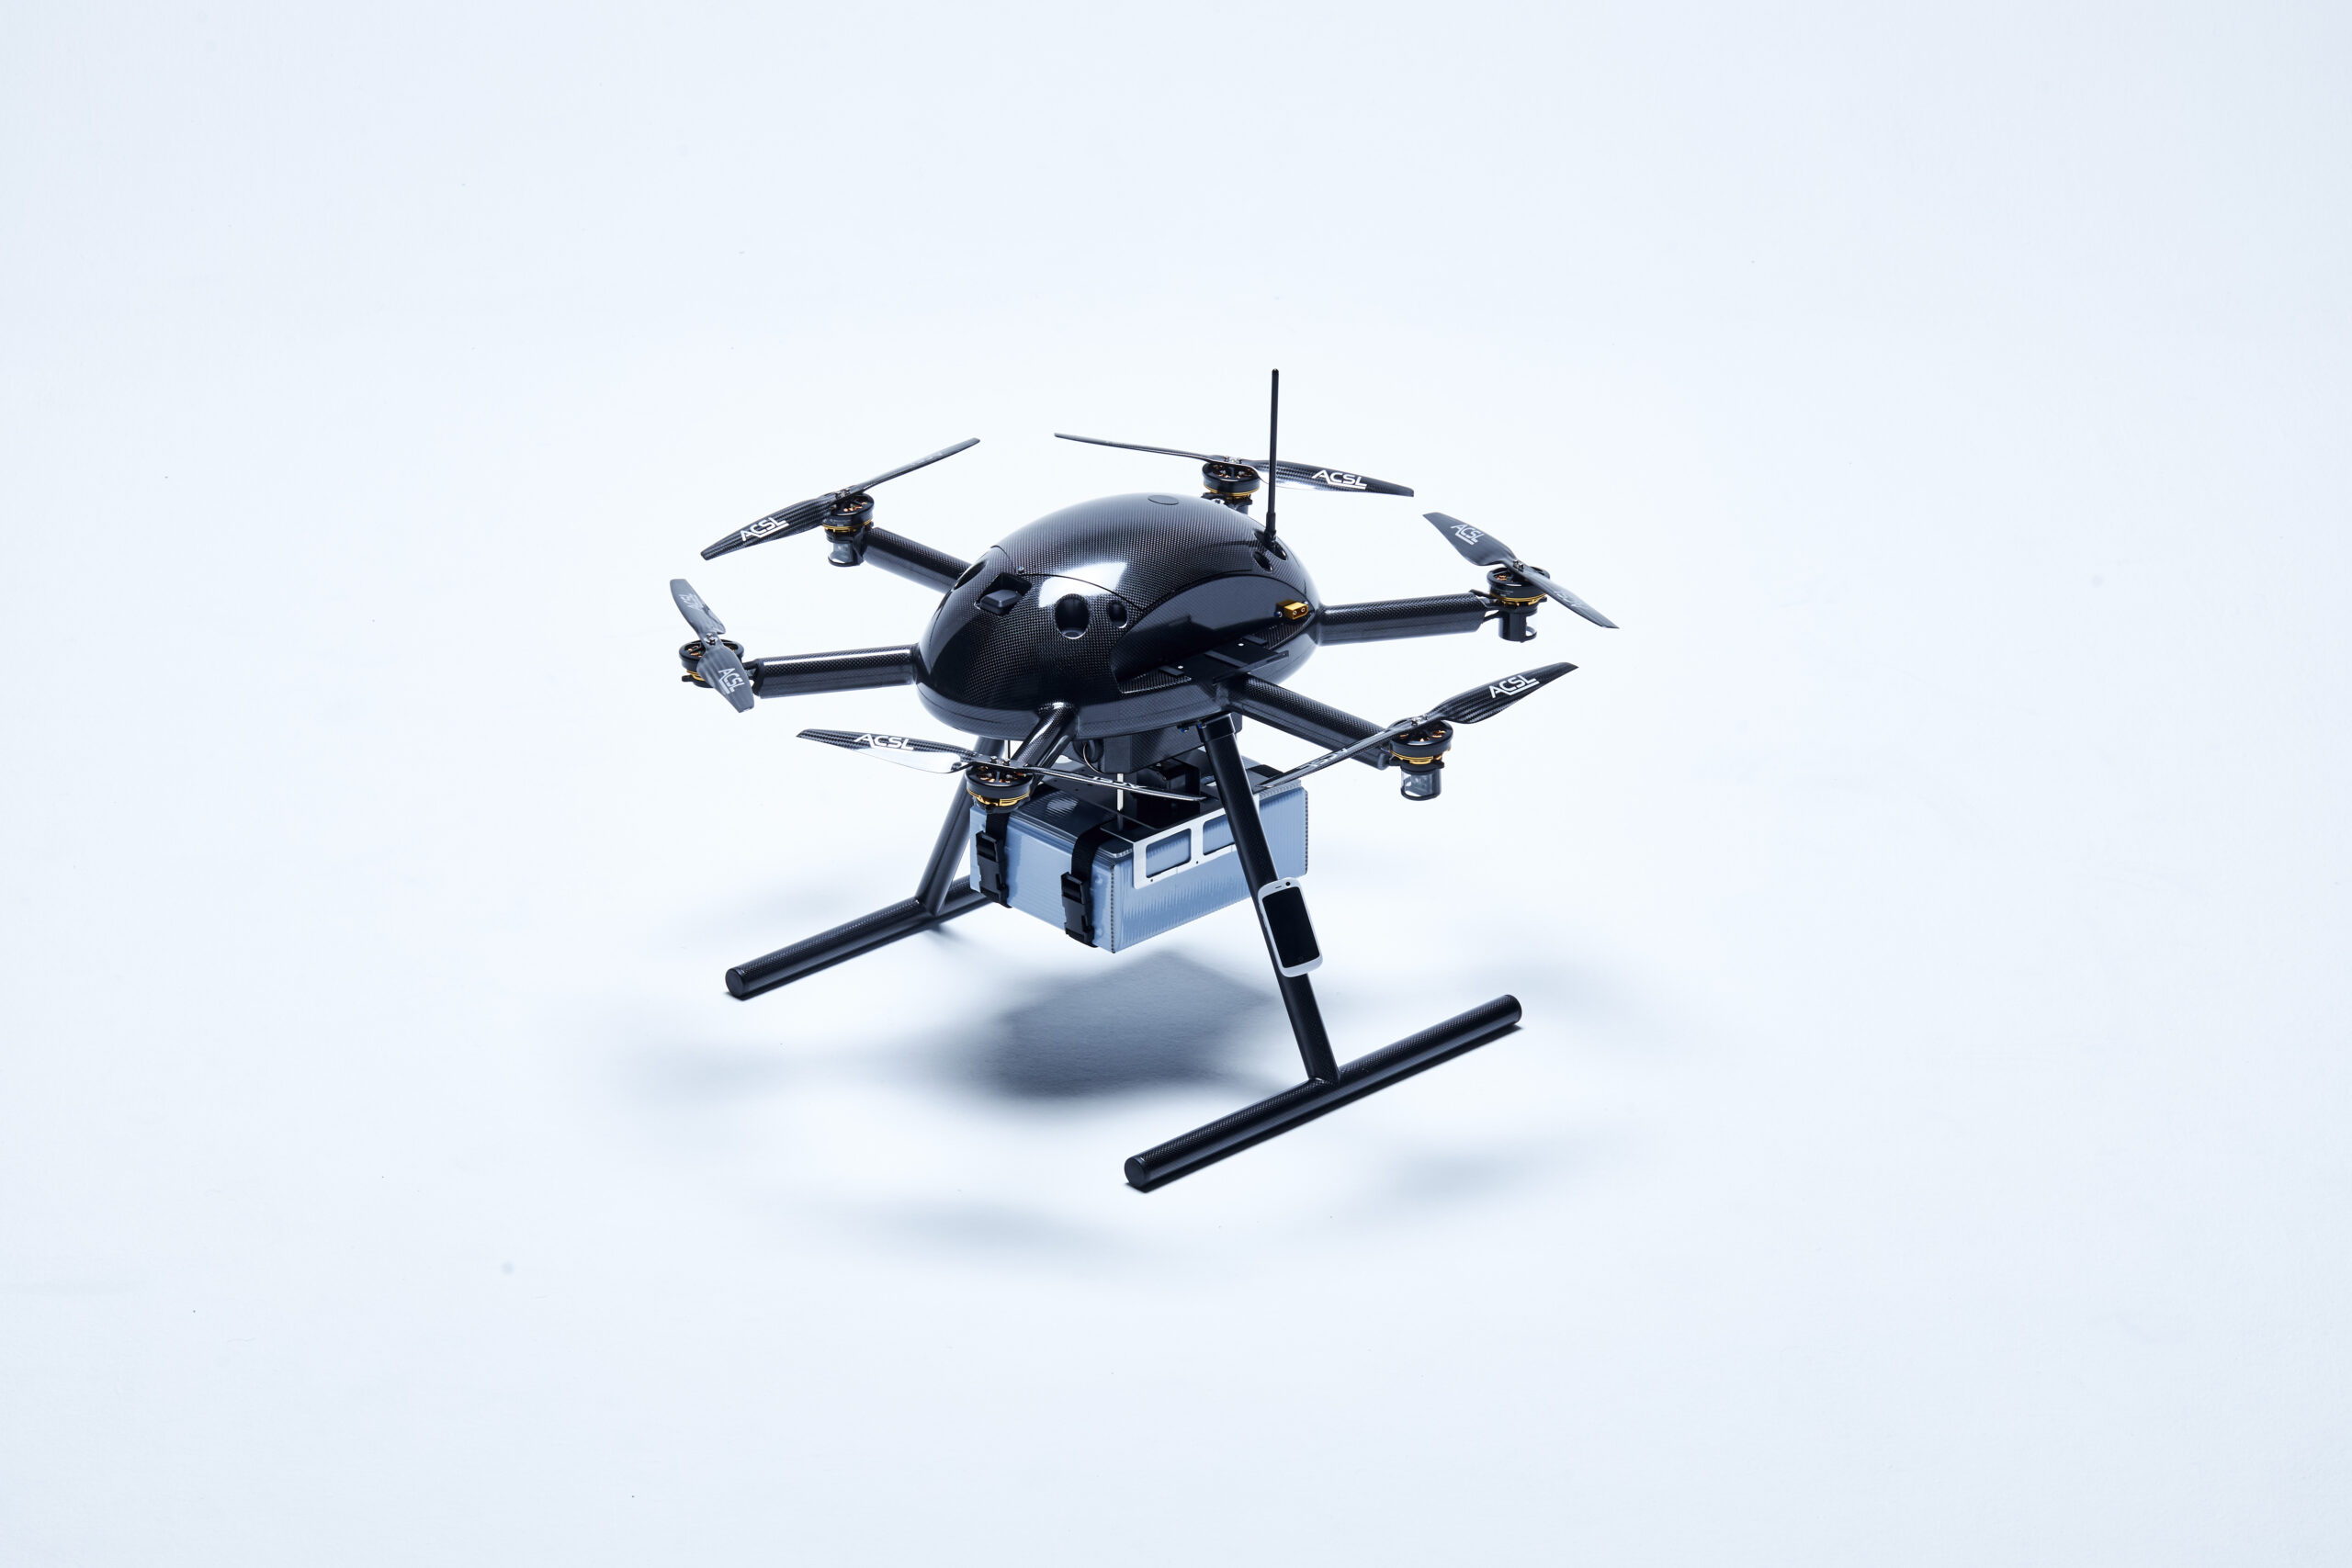
\includegraphics[width=\textwidth]{partes/img/PF2.jpg}
        \caption{PF2}
        \label{fig:pf2}
    \end{subfigure}
    \hfill
    \begin{subfigure}[b]{0.45\textwidth}
        \centering
        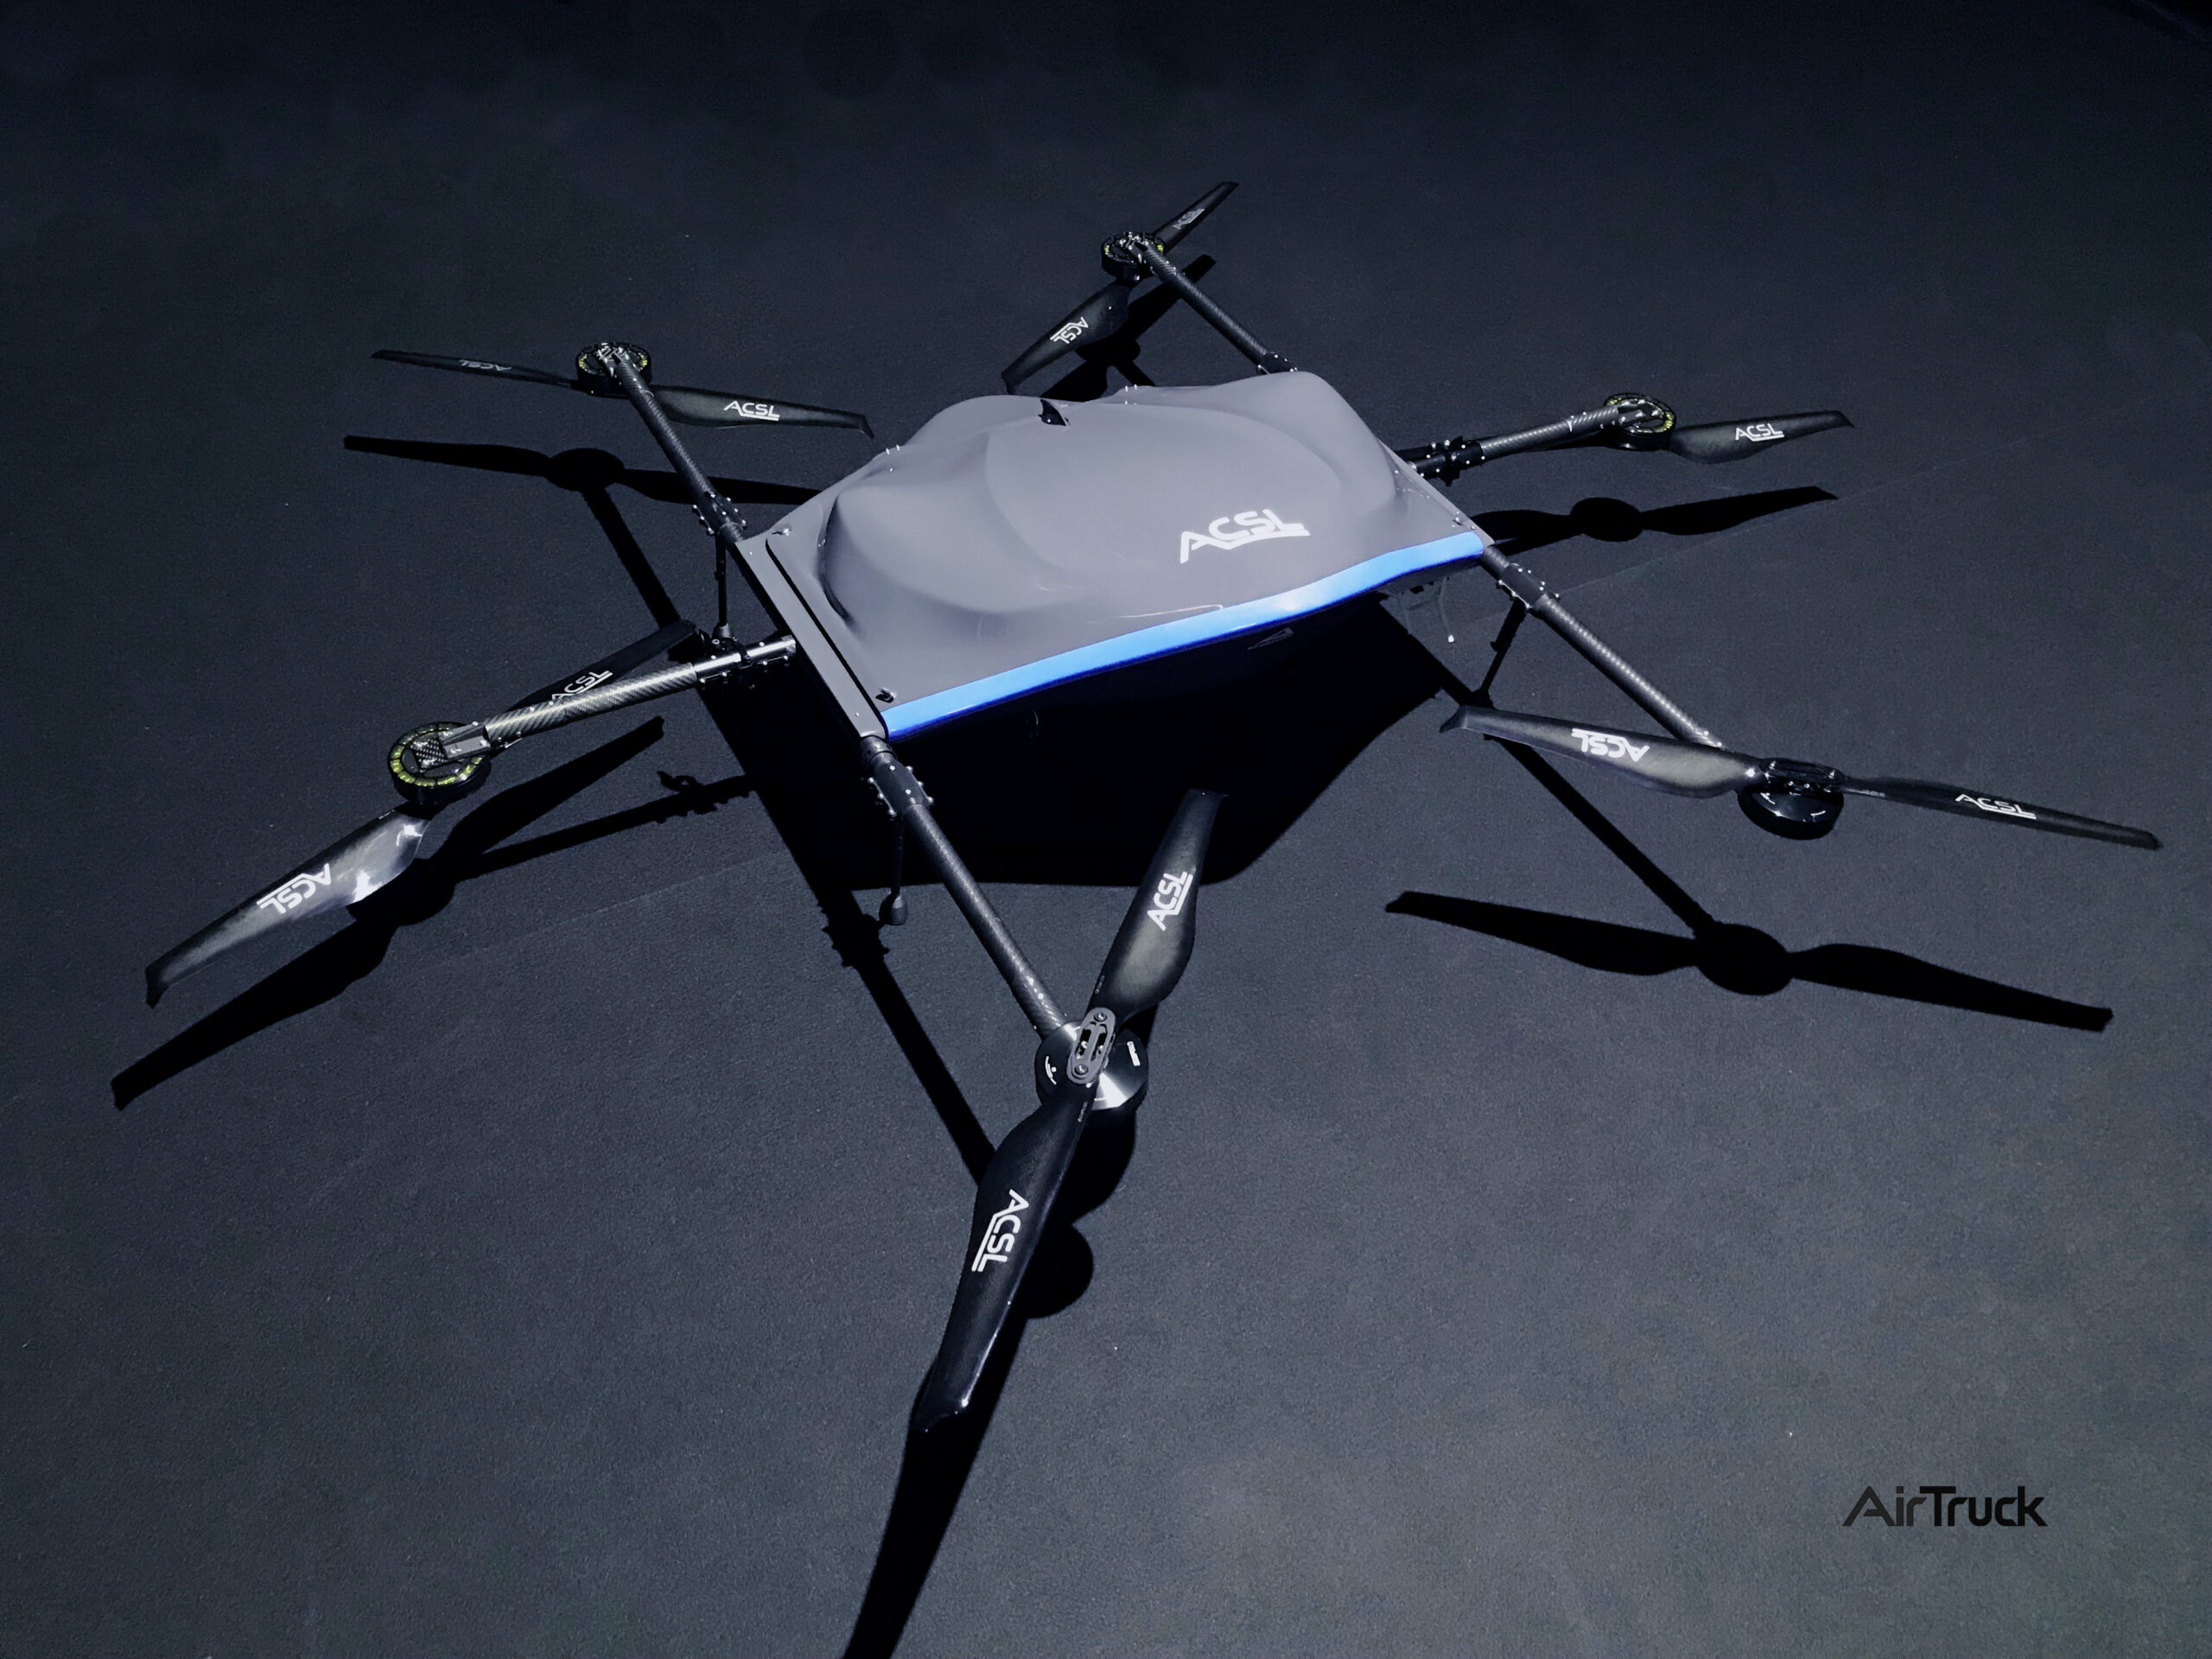
\includegraphics[width=\textwidth]{partes/img/AirTruck.jpg}
        \caption{AirTruck}
        \label{fig:AirTruck}
    \end{subfigure}
    \break
    \begin{subfigure}[b]{0.45\textwidth}
        \centering
        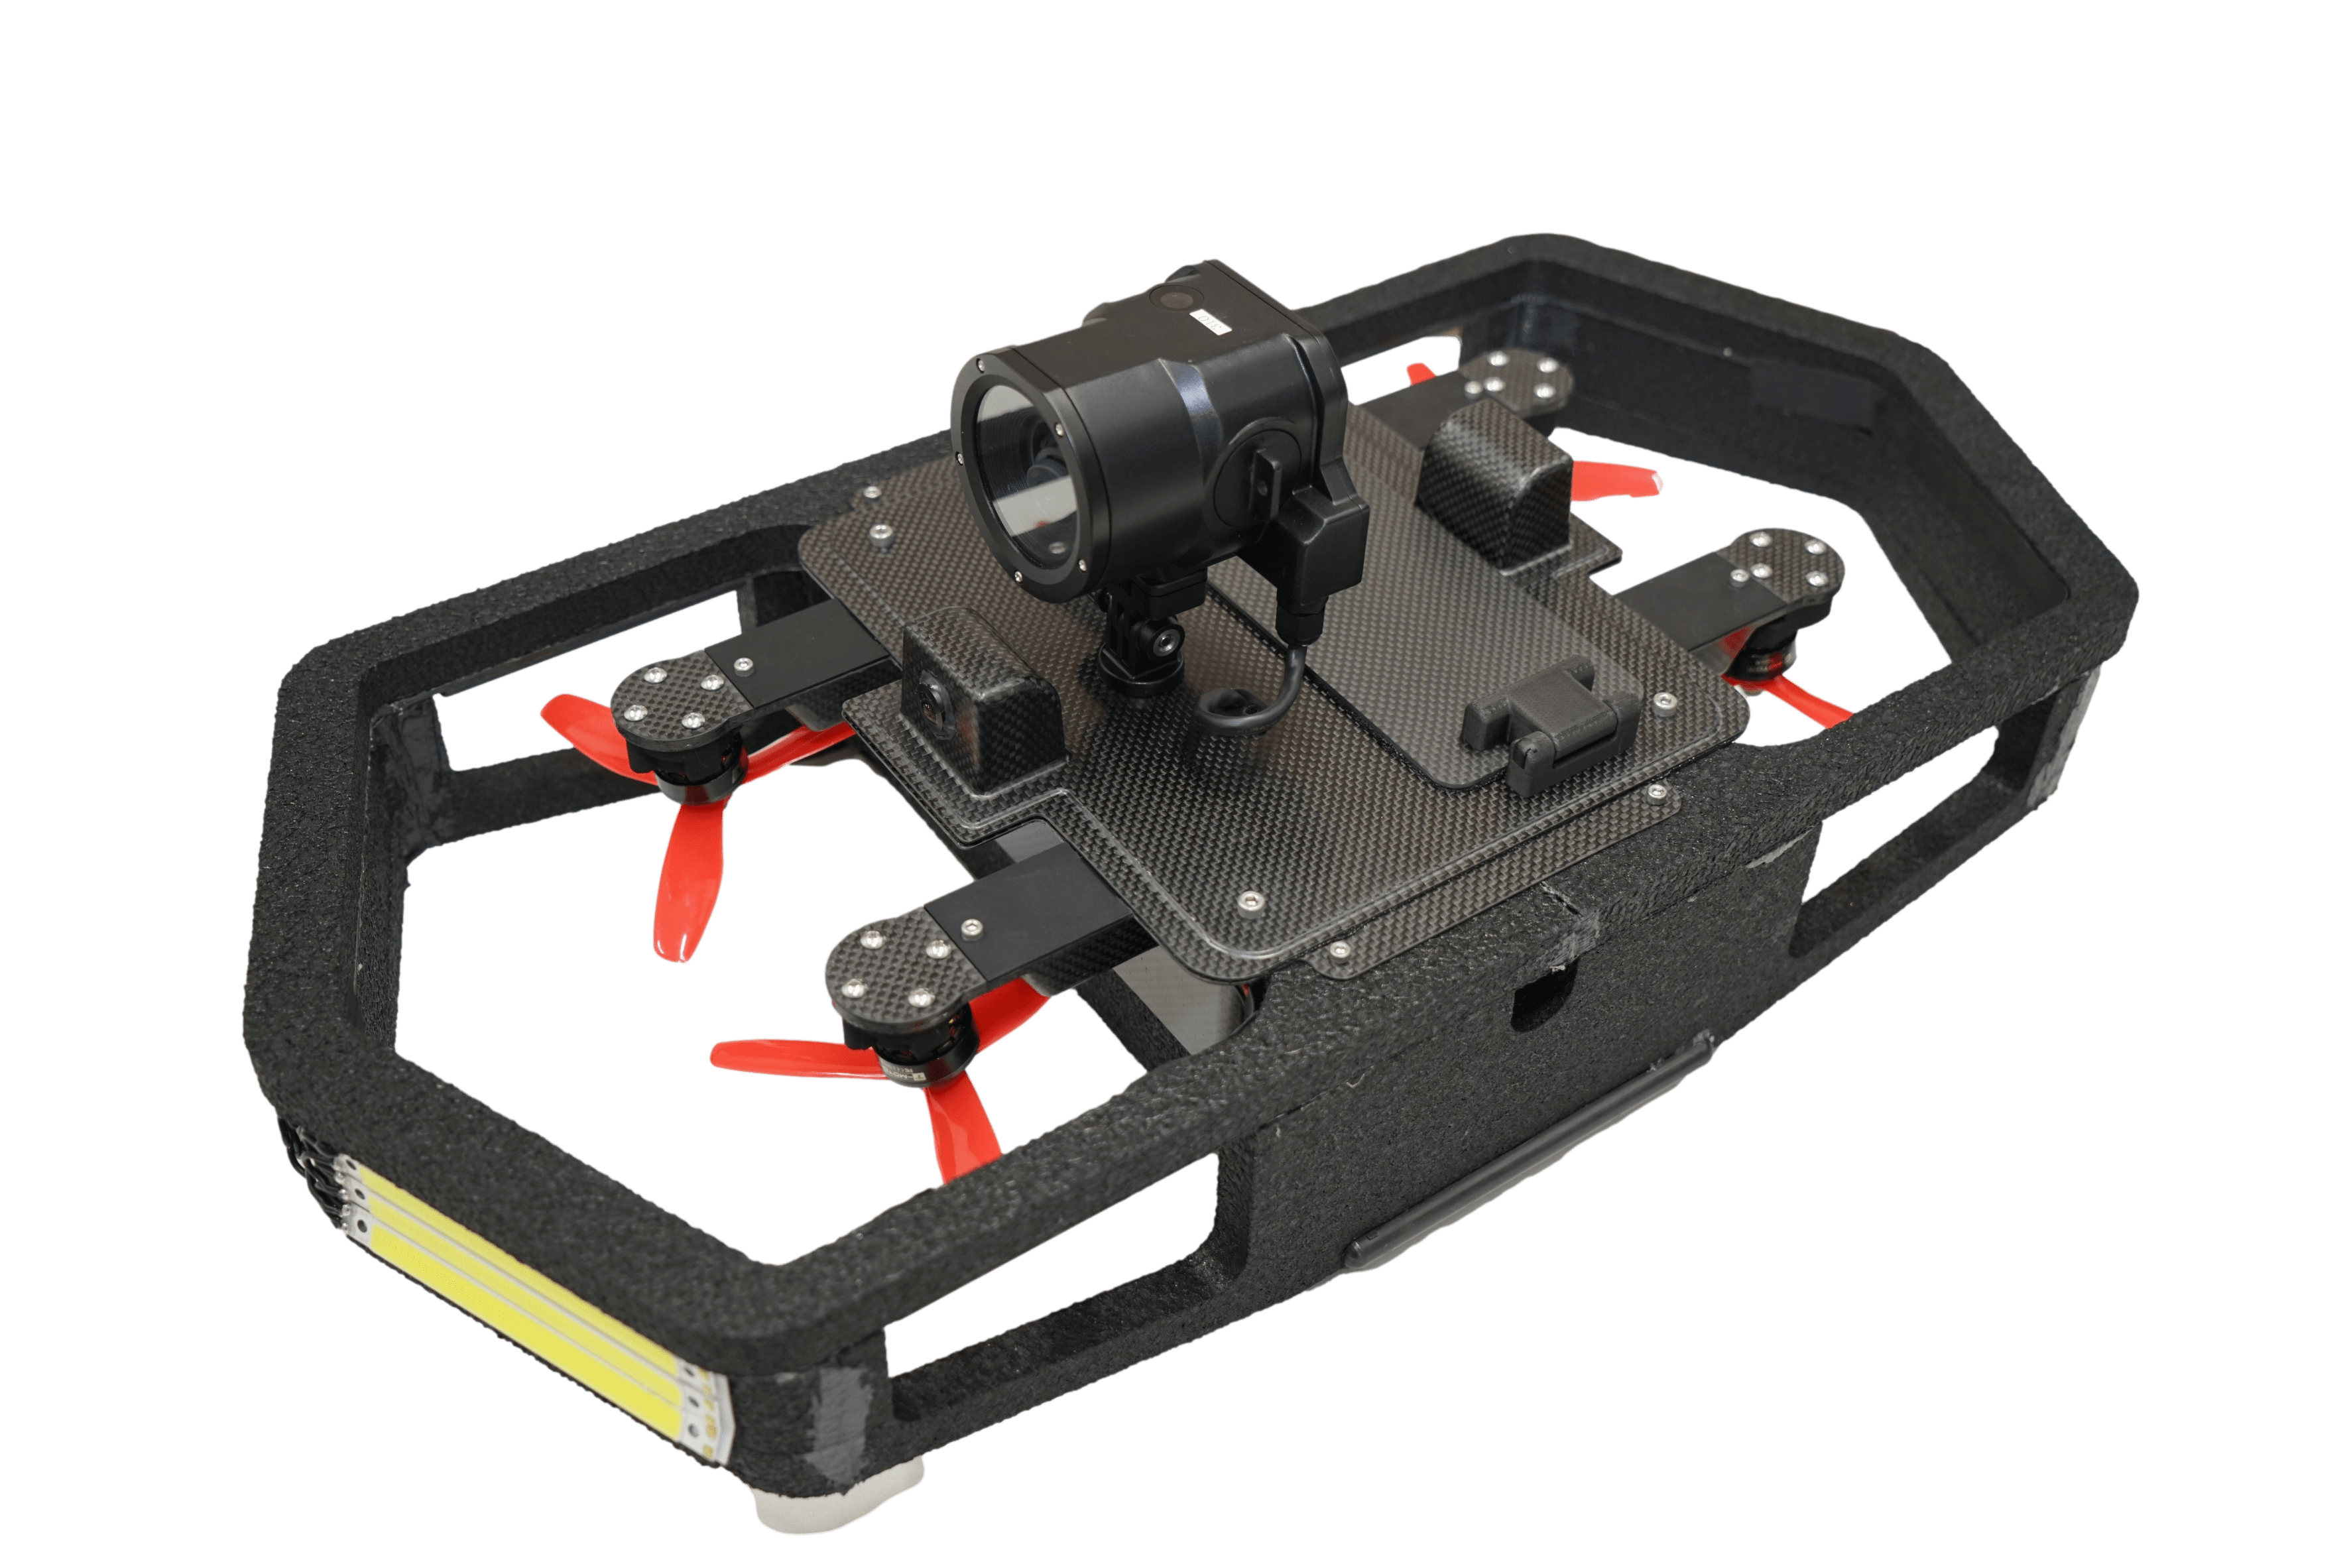
\includegraphics[width=\textwidth]{partes/img/Fi4.png}
        \caption{Fi4}
        \label{fig:Fi4}
    \end{subfigure}
    \hfill
    \begin{subfigure}[b]{0.45\textwidth}
        \centering
        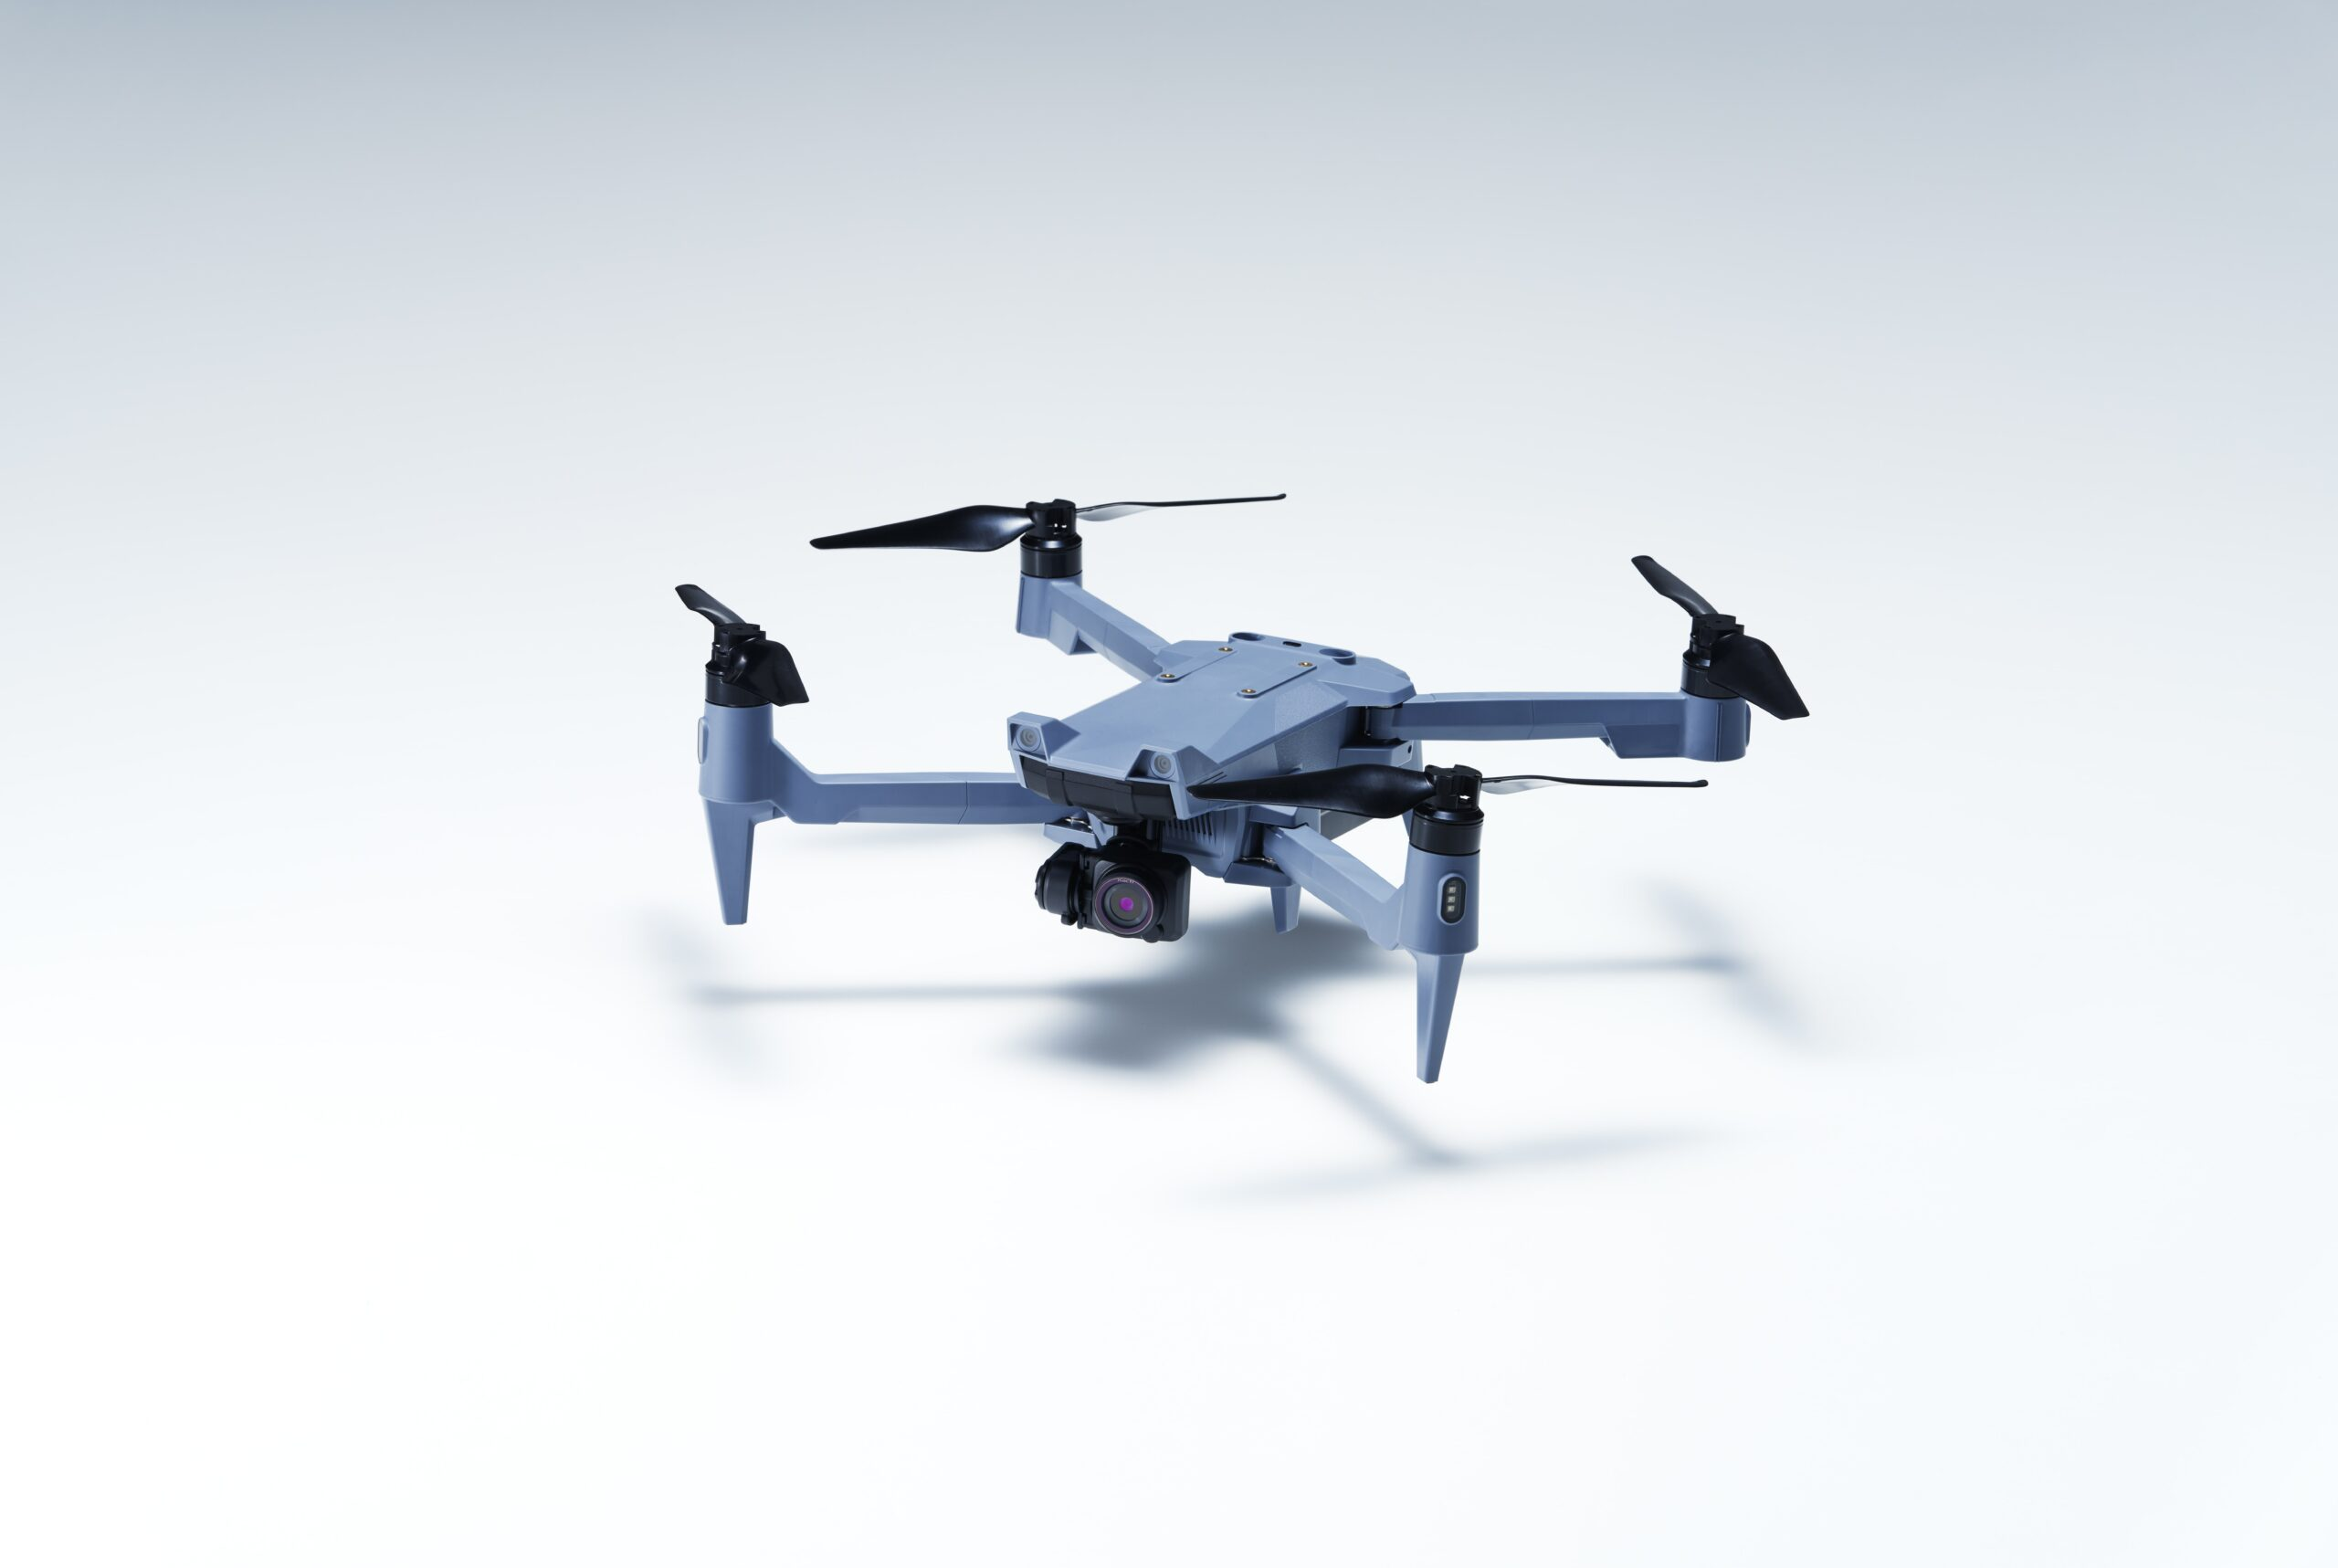
\includegraphics[width=\textwidth]{partes/img/SOTEN.jpg}
        \caption{SOTEN}
        \label{fig:SOTEN_ACSL}
    \end{subfigure}
    \hfill
    
    \caption [Algunos productos de ACSL]{Algunos productos de ACSL. \textbf{(a)} \textbf{PF2}: Un dron con capacidad autónoma de seis rotores utilizado para aplicaciones de entrega de paquetes (\textit{delivery}), inspección y patrullaje en desastres naturales. \textbf{(b)} \textbf{AirTruck}: Un dron autónomo de seis rotores con capacidad de carga y vuelo superior utilizado para operaciones de logística. \textbf{(c)} \textbf{Fi4}: Un dron autónomo dedicado a la inspección de espacios confinados (tuberías, ductos de ventilación, entre otros). \textbf{(d)} \textbf{SOTEN}: Un dron pequeño de cuatro rotores dedicado a la fotografía aérea con capacidad autónoma utilizado para tareas de inspección, vigilancia y rescate. }
    \label{fig:acsl-products}
\end{figure}


Este trabajo se desarrolló bajo la supervisión del Equipo de Inteligencia de Máquinas (del inglés \textit{Machine Intelligence Team}) de ACSL, contando con Niklas Bergstroem, lider del Equipo de Inteligencia de Máquinas, como encargado de asesorar el desarrollo del trabajo. Gracias a los miembros del Equipo de Inteligencia de Máquinas de ACSL, este trabajo pudo ser desarrollado e implementado haciendo el uso de las plataformas y recursos disponibles.
